\chapter{Fisiología renal y osmorregulación}\label{ch:b3:renal-osmoregulation}

Los riñones filtran ciento ochenta litros de plasma al día ---todo el
volumen sanguíneo cada media hora--- y devuelven todo salvo un litro y
medio, tras haber retirado la urea y haber ajustado la sal, el ácido y
el agua a menos de un uno por ciento de lo que el cuerpo necesita,
conservando cada gramo de glucosa. Una rata canguro del desierto no
bebe nunca: vive del agua que su metabolismo fabrica a partir de
semillas secas y excreta una orina cinco veces más concentrada que el
agua de mar. Un pez marino bebe sin cesar y expulsa la sal por las
branquias; un pez de agua dulce no bebe nunca y bombea sal hacia
dentro. El problema que todos resuelven es el mismo: mantener constante
la composición del líquido que rodea a las células mientras comer,
beber y respirar la perturban, y desechar el nitrógeno sin desechar
demasiada agua. Este capítulo trata el riñón de los mamíferos como
ejemplo desarrollado ---la filtración, la aritmética del aclaramiento,
el truco de la contracorriente que concentra la orina y las hormonas
que fijan los mandos--- y después el abanico de soluciones a lo largo
del reino animal.

\section{El problema}

\begin{definition}[La osmorregulación]\label{def:b3:renal-osmoregulation:problem}
\index{osmolaridad}\index{presión osmótica}\index{líquido extracelular}\index{osmoconformador}\index{osmorregulador}
La \emph{osmolaridad} de una disolución es su concentración total de
partículas disueltas (en osmoles por litro); fija la \emph{presión
osmótica}, $\Pi = cRT$ en disoluciones diluidas, que impulsa el agua a
través de cualquier membrana que deje pasar agua pero no soluto. Los
líquidos corporales de un mamífero se sitúan en torno a
\qty{300}{mOsm/L} ---el \qty{40}{\%} de la masa corporal dentro de las
células y el \qty{20}{\%} fuera, el \emph{líquido extracelular}, del
que una cuarta parte es plasma--- y las células se hinchan o se encogen
en segundos si el exterior cambia, puesto que sus membranas dejan pasar
el agua libremente. Un \emph{osmoconformador} (la mayoría de los
invertebrados marinos, los tiburones) mantiene sus líquidos a la
osmolaridad del mar y regula solo su composición; un
\emph{osmorregulador} (vertebrados, insectos, animales de agua dulce)
mantiene su osmolaridad constante frente al medio, lo que cuesta
energía en proporción al gradiente. La segunda tarea, acoplada a la
primera, es deshacerse del nitrógeno de la degradación de las
proteínas: como \emph{amoníaco} en agua abundante (peces), como
\emph{urea}, soluble y no tóxica pero que necesita agua para
arrastrarla (mamíferos), o como \emph{ácido úrico}, una pasta excretada
casi seca (aves, reptiles, insectos).
\end{definition}

\section{La nefrona y la filtración}

\begin{definition}[La nefrona]\label{def:b3:renal-osmoregulation:nephron}
\index{nefrona}\index{glomérulo}\index{túbulo proximal}\index{asa de Henle}\index{tubo colector}
Cada riñón humano alberga aproximadamente un millón de \emph{nefronas}.
La sangre entra en un \emph{glomérulo}, un ovillo de capilares dentro
de la cápsula de Bowman, cuyas paredes ---endotelio fenestrado,
membrana basal y los diafragmas de hendidura entre los pies de los
podocitos--- dejan pasar agua y todo soluto por debajo de unos
\qty{60}{kDa}, pero retienen las proteínas y las células. El filtrado
fluye por el \emph{túbulo proximal}, que reabsorbe dos tercios del agua
y de la sal y toda la glucosa y los aminoácidos; baja y sube por el
\emph{asa de Henle}, que penetra en la médula y construye el gradiente
de concentración de la sección siguiente; atraviesa el \emph{túbulo
distal}, donde se ajusta la sal; y llega al \emph{tubo colector}, donde
la vasopresina fija el contenido final de agua mientras el tubo
atraviesa la médula camino de la pelvis. La sangre que sale del
glomérulo entra en un segundo lecho capilar alrededor de los túbulos,
que recoge lo que estos reabsorben.
\end{definition}

\begin{omfigure}
\begin{tikzpicture}[every node/.style={font=\scriptsize}, >=stealth]
  % cortex/medulla background
  \fill[omDef!6] (-0.5,0) rectangle (11.5,3.6); \fill[omProp!8] (-0.5,-3.4) rectangle (11.5,0);
  \node[right, gray] at (-0.4,3.4) {corteza}; \node[right, gray] at (-0.4,-3.2) {médula};
  % glomerulus
  \draw[thick, omThm, fill=omThm!20] (0.8,2.6) circle (0.55); \node[below, align=center] at (0.25,2.0) {glomérulo:\\filtración,\\\qty{180}{L/d}};
  % proximal tubule
  \draw[very thick, omDef] (1.35,2.6) .. controls (2.2,3.3) and (2.8,2.0) .. (3.2,2.6) .. controls (3.5,3.1) and (3.9,2.2) .. (4.2,2.6);
  \node[below, align=center] at (2.65,2.05) {túbulo proximal:\\\qty{67}{\%} del Na$^{+}$ y del agua,\\toda la glucosa, los aminoácidos,\\HCO$_3^-$};
  % loop of Henle
  \draw[very thick, omDef] (4.2,2.6) -- (4.2,-2.8) arc[start angle=180, end angle=360, radius=0.4] -- (5.0,2.6);
  \node[left, align=right] at (4.1,-1.0) {rama descendente:\\sale agua};
  \node[right, align=left] at (5.1,-1.6) {rama ascendente:\\se bombea NaCl,\\no agua};
  \node[right, align=left, omProp!80!black] at (5.1,-0.2) {\qty{25}{\%} del Na$^{+}$};
  % distal tubule
  \draw[very thick, omDef] (5.0,2.6) .. controls (5.4,3.2) and (6.0,2.0) .. (6.4,2.6) .. controls (6.8,3.1) .. (7.2,2.6);
  \node[above, align=center] at (6.0,3.1) {túbulo distal: Na$^{+}$ (aldosterona),\\Ca$^{2+}$, secreción de K$^{+}$};
  % collecting duct
  \draw[very thick, omMeth!70!black] (7.2,2.6) -- (7.8,2.6) -- (7.8,-3.2);
  \node[right, align=left] at (7.9,-1.2) {tubo colector:\\agua (vasopresina,\\acuaporina-2),\\urea, H$^{+}$;\\salen \qty{1.5}{L/d}};
  \draw[->, thick, omMeth!70!black] (7.8,-3.2) -- (7.8,-3.6);
  % osmolarity scale on the right
  \foreach \y/\c in {2.6/300, 0.0/600, -1.4/900, -2.8/1200} { \node[left, omProp!80!black, font=\tiny] at (11.4,\y) {\c\ mOsm}; }
  \draw[->, omProp!80!black] (11.4,2.9) -- (11.4,-3.1); \node[above, omProp!80!black, font=\tiny, align=center] at (11.4,3.0) {osmolaridad\\intersticial};
\end{tikzpicture}

{\small Una \omterm{def:b3:renal-osmoregulation:nephron}{nefrona} desplegada. La filtración en la corteza; la
reabsorción masiva en el \omterm{def:b3:renal-osmoregulation:nephron}{túbulo proximal}; el \omterm{def:b3:renal-osmoregulation:nephron}{asa de Henle} que se hunde
en la médula, donde el intersticio se vuelve más salado con la
profundidad; el \omterm{def:b3:renal-osmoregulation:nephron}{tubo colector} que vuelve a atravesar ese gradiente y
cede agua si la vasopresina lo permite.}
\end{omfigure}

\begin{theorem}[Filtración y aclaramiento]\label{thm:b3:renal-osmoregulation:clearance}
\index{fuerzas de Starling}\index{tasa de filtración glomerular}\index{aclaramiento}\index{inulina}\index{creatinina}
El filtrado atraviesa la pared glomerular a un ritmo que fijan las
\emph{\omterm{thm:b3:renal-osmoregulation:clearance}{fuerzas de Starling}}: la presión hidrostática del capilar
$P_{\text{CG}}$ empuja el líquido hacia fuera, la presión hidrostática
del espacio de Bowman $P_{\text{EB}}$ y la presión oncótica de las
proteínas plasmáticas $\pi_{\text{CG}}$ lo retienen, y
\[
\text{TFG} = K_{f}\,\bigl(P_{\text{CG}} - P_{\text{EB}} - \pi_{\text{CG}}\bigr)
\approx K_{f}\,(55 - 15 - 30)\ \unit{mmHg} = K_{f}\times \qty{10}{mmHg},
\]
la \emph{\omterm{thm:b3:renal-osmoregulation:clearance}{tasa de filtración glomerular}}, de unos \qty{125}{mL/min} en
un adulto. Para cualquier sustancia $x$ de concentración plasmática
$P_{x}$, concentración urinaria $U_{x}$ y flujo de orina $V$, el
\emph{aclaramiento}
\[
C_{x} = \frac{U_{x}\,V}{P_{x}}
\]
es el volumen de plasma depurado de $x$ por unidad de tiempo. Si $x$ se
filtra libremente y no se reabsorbe ni se secreta (la inulina y, casi,
la creatinina), $C_{x} = \text{TFG}$; si se elimina por completo del
plasma que pasa por el riñón (el paraaminohipurato a dosis baja),
$C_{x}$ es igual al flujo plasmático renal; un aclaramiento por debajo
de la TFG significa reabsorción neta, y por encima, secreción neta, y
la carga filtrada $\text{TFG}
\times P_{x}$ menos la excreción $U_{x}V$ es la cantidad reabsorbida.
\end{theorem}
\begin{proof}
La filtración es una ultrafiltración a través de una pared porosa: el
flujo es proporcional a la presión neta que la atraviesa, y la presión
neta es la hidrostática hacia fuera menos la hidrostática y la oncótica
hacia dentro (Starling), siendo despreciable la presión oncótica del
filtrado, que no contiene proteína. El aclaramiento: en la unidad de
tiempo el riñón excreta $U_{x}V$ de $x$; el volumen de plasma que
contenía esa cantidad es $U_{x}V/P_{x}$. Para una sustancia que solo se
filtra, lo excretado es lo filtrado, $\text{TFG}\times P_{x} = U_{x}V$,
de donde $C_{x} = \text{TFG}$. Para una extraída por completo, todo el
$x$ del plasma que circula, $\text{FPR}\times P_{x}$, se excreta, de
donde $C_{x} = \text{FPR}$. El balance de materia da la cantidad
reabsorbida.
\end{proof}

\begin{example}[Aclaramientos en números]\label{ex:b3:renal-osmoregulation:numbers}
La inulina, infundida hasta un nivel plasmático de \qty{1}{mg/mL},
aparece en la orina a \qty{125}{mg/mL} con un flujo de \qty{1}{mL/min}: $C = 125\times 1/1 =
\qty{125}{mL/min}$, la TFG, \qty{180}{L/d}. El paraaminohipurato da
\qty{650}{mL/min}, el flujo plasmático; con un hematocrito de $0.45$ el
flujo sanguíneo renal es de \qty{1.2}{L/min}, la quinta parte del gasto
cardíaco para el \qty{0.5}{\%} de la masa corporal, y la fracción de
filtración, $125/650 = 0.19$. Urea: plasma \qty{5}{mmol/L}, orina
\qty{300}{mmol/L} a \qty{1}{mL/min} ---aclaramiento \qty{60}{mL/min},
la mitad de la TFG, de modo que se reabsorbe la mitad de la urea
filtrada. Glucosa: aclaramiento cero a niveles plasmáticos normales, y
cada molécula de los \qty{180}{g} filtrados al día devuelta. La
creatinina, fabricada por el músculo a ritmo constante y solo filtrada,
es la medida clínica de la TFG: cuando la TFG se reduce a la mitad, la
creatinina plasmática se duplica, sin recoger orina alguna.
\end{example}

\begin{method}[Medir la función renal]\label{met:b3:renal-osmoregulation:gfr}
\index{medida de la tasa de filtración glomerular}
(1) Para un valor de investigación, infúndase inulina hasta un nivel
plasmático estable, recójase orina cronometrada, mídanse ambas y
calcúlese $UV/P$. (2) En la clínica, mídase la creatinina plasmática y
estímese la TFG a partir de ella con una fórmula que corrige por edad,
sexo y tamaño corporal; la estimación es lo que define los estadios de
la enfermedad renal crónica (una TFG por debajo de \qty{60}{mL/min}
durante tres meses). (3) Pruébese la selectividad del filtro midiendo
la albúmina en la orina ---normalmente por debajo de \qty{30}{mg/d};
más significa una barrera con fugas, el signo más temprano del daño
renal diabético. (4) Pruébese la capacidad de concentración privando de
agua durante la noche y midiendo la \omterm{def:b3:renal-osmoregulation:problem}{osmolaridad} de la orina, que
debería superar los \qty{800}{mOsm/L}; el fracaso en concentrar con una
TFG normal apunta al \omterm{def:b3:renal-osmoregulation:nephron}{tubo colector} o a la vasopresina.
\end{method}

\begin{omfigure}
\begin{tikzpicture}
\begin{axis}[
  width=0.68\linewidth, height=5.6cm,
  axis x line=bottom, axis y line=left,
  xmin=0, xmax=800, ymin=0, ymax=700,
  xlabel={glucosa plasmática (mg/dL)}, ylabel={mg/min},
  xlabel style={font=\small, at={(axis description cs:0.5,-0.12)}, anchor=north}, ylabel style={font=\small},
  tick label style={font=\small}, xtick={0,100,200,300,400,600,800}, ytick={0,200,375,600},
  clip=false,
]
\addplot[very thick, omDef, domain=0:800, samples=2] {1.25*x};
\addplot[very thick, omMeth!70!black, domain=0:200, samples=2] {1.25*x};
\addplot[very thick, omMeth!70!black, smooth] coordinates {(200,250) (250,300) (300,340) (350,365) (400,375) (800,375)};
\addplot[very thick, omThm, domain=0:180, samples=2] {0};
\addplot[very thick, omThm, smooth] coordinates {(180,0) (250,12) (300,35) (350,72) (400,125) (800,625)};
\draw[dashed, gray] (axis cs:180,0) -- (axis cs:180,700); \node[font=\scriptsize, gray, anchor=north west] at (axis cs:185,560) {umbral};
\draw[dashed, gray] (axis cs:0,375) -- (axis cs:800,375);
\node[font=\scriptsize, omDef, anchor=south east] at (axis cs:480,620) {filtrada: TFG $\times$ P};
\node[font=\scriptsize, omMeth!70!black, anchor=south west, align=left] at (axis cs:660,395) {reabsorbida:\\$T_{m} = \qty{375}{mg/min}$};
\node[font=\scriptsize, omThm, anchor=north west] at (axis cs:520,300) {excretada};
\end{axis}
\end{tikzpicture}

{\small La curva de titulación de la glucosa. La carga filtrada crece
con el nivel plasmático; los transportadores del \omterm{def:b3:renal-osmoregulation:nephron}{túbulo proximal} la
reabsorben toda hasta su máximo $T_{m}$; por encima del umbral, hacia
\qty{180}{mg/dL} (\qty{10}{mmol/L}), la glucosa se derrama a la orina
---el azúcar en la orina de la diabetes no tratada.}
\end{omfigure}

\section{Concentrar la orina}

\begin{proposition}[El multiplicador por contracorriente]\label{prop:b3:renal-osmoregulation:countercurrent}
\index{multiplicación por contracorriente}\index{efecto simple}\index{vasopresina}\index{acuaporina}\index{reciclado de urea}
El \omterm{def:b3:renal-osmoregulation:nephron}{asa de Henle} construye un gradiente de \omterm{def:b3:renal-osmoregulation:problem}{osmolaridad} desde los
\qty{300}{mOsm/L} de la corteza hasta los \qty{1200}{mOsm/L} de la
punta de la médula, sin que ninguna célula bombee contra más que una
fracción de él. La rama ascendente gruesa bombea NaCl desde su líquido
hacia el intersticio y es impermeable al agua, de modo que en cada
nivel deja el intersticio unos \qty{200}{mOsm/L} más salado que su
propio contenido ---el \emph{\omterm{prop:b3:renal-osmoregulation:countercurrent}{efecto simple}}. La rama descendente es
permeable al agua y se equilibra con el intersticio, de modo que el
líquido que baja se vuelve más salado a medida que desciende y entrega
al recodo un líquido ya concentrado, del que bombea entonces la rama
ascendente; el líquido que sube se vuelve más diluido que el
intersticio en cada nivel y abandona el asa a \qty{100}{mOsm/L},
hipotónico. El flujo a contracorriente convierte un efecto transversal
pequeño en un gradiente longitudinal grande: el líquido más salado del
recodo se hizo a partir de un líquido que ya era salado, etapa sobre
etapa. El \omterm{def:b3:renal-osmoregulation:nephron}{tubo colector} recorre después ese gradiente hacia abajo. Sin
\emph{vasopresina} (hormona antidiurética) su pared es impermeable al
agua y cada hora sale un litro o más de orina diluida; con ella, se
insertan canales de \emph{acuaporina-2} en la membrana luminal, el agua
sale gradiente abajo hacia la médula y la orina alcanza la \omterm{def:b3:renal-osmoregulation:problem}{osmolaridad}
de la punta, \qty{1200}{mOsm/L}. La urea, reabsorbida desde el tubo
interno y atrapada en la médula, aporta la mitad de la \omterm{def:b3:renal-osmoregulation:problem}{osmolaridad} de
la punta, y los vasos rectos, ellos mismos en contracorriente, retiran
el agua reabsorbida sin lavar el gradiente.
\end{proposition}

\begin{proof}[Evidencia]
Wirz, Hargitay y Kuhn (1951) congelaron riñones de rata y midieron el
punto de fusión del líquido en cortes que iban de la corteza a la
papila: la \omterm{def:b3:renal-osmoregulation:problem}{osmolaridad} subía sin cesar con la profundidad y alcanzaba
en la punta el valor de la orina ---el gradiente que exigía la teoría
del multiplicador por contracorriente (Kuhn, químico físico, 1942). La
micropunción de los túbulos (Gottschalk, 1959) halló después
hipertónico el líquido del recodo del asa e hipotónico el que salía de
la rama ascendente, y el líquido del \omterm{def:b3:renal-osmoregulation:nephron}{tubo colector} igualado al
intersticio en cada nivel cuando había vasopresina. Los roedores del
desierto con las asas más largas tenían los gradientes más empinados y
la orina más concentrada.
\end{proof}

\begin{omfigure}
\begin{tikzpicture}[every node/.style={font=\scriptsize}, >=stealth]
  % loop
  \draw[very thick, omDef] (0,3.2) -- (0,-0.4) arc[start angle=180, end angle=360, radius=0.7] -- (1.4,3.2);
  \draw[very thick, omDef] (0.35,3.2) -- (0.35,-0.4) arc[start angle=180, end angle=360, radius=0.35] -- (1.05,3.2);
  % interstitial osmolarity bands
  \foreach \y/\c/\col in {2.8/300/10, 2.0/500/25, 1.2/700/40, 0.4/900/55, -0.4/1100/70, -1.0/1200/80} { \fill[omProp!\col, opacity=0.5] (-2.2,\y-0.4) rectangle (-0.2,\y+0.4); \node[left, font=\tiny] at (-2.25,\y) {\c}; }
  \node[left, align=right, font=\tiny] at (-2.25,3.35) {intersticio\\(mOsm/L)};
  % arrows: water out of descending, NaCl out of ascending
  \foreach \y in {2.4,1.6,0.8,0.0} { \draw[->, thick, omDef!70!black] (0.15,\y) -- (-0.4,\y); }
  \node[left, omDef!70!black, font=\tiny] at (-0.45,2.4) {H$_2$O};
  \foreach \y in {2.4,1.6,0.8,0.0} { \draw[->, thick, omThm] (1.25,\y) -- (1.9,\y); }
  \node[right, omThm, font=\tiny] at (1.5,2.85) {NaCl bombeado};
  % fluid osmolarity labels inside limbs
  \node[above] at (0.17,3.25) {entran \qty{300}{}}; \node[above] at (1.22,3.25) {salen \qty{100}{}};
  \node[font=\tiny] at (0.7,-1.35) {1200 en el recodo};
  \node[below, align=center] at (0.2,-1.7) {rama descendente: sale agua,\\el líquido se concentra; rama ascendente:\\sale sal, el líquido se diluye};
  % collecting duct
  \draw[very thick, omMeth!70!black] (4.2,3.2) -- (4.2,-1.4); \node[above, align=center] at (4.2,3.25) {tubo colector};
  \foreach \y in {2.4,1.6,0.8,0.0,-0.8} { \draw[->, thick, omMeth!70!black] (4.1,\y) -- (3.5,\y); }
  \node[right, align=left, font=\tiny] at (4.3,1.2) {con vasopresina:\\se inserta acuaporina-2,\\el agua sale\\gradiente abajo};
  \node[below, align=center] at (4.2,-1.5) {orina hasta\\\qty{1200}{mOsm/L}};
  % single effect note
  \node[right, align=left] at (6.4,2.6) {el efecto simple: la rama ascendente\\mantiene el intersticio $\sim\qty{200}{mOsm/L}$\\por encima de su propio líquido en cada nivel;\\el flujo a contracorriente apila los efectos\\en un gradiente de \qty{900}{mOsm/L}\\de la corteza a la papila};
\end{tikzpicture}

{\small El multiplicador por contracorriente. La sal bombeada desde la
rama ascendente vuelve hipertónico el intersticio; el agua extraída de
la rama descendente concentra el líquido antes de que alcance la bomba;
el flujo en sentidos opuestos apila una pequeña diferencia transversal
en un gradiente cuádruple, que el \omterm{def:b3:renal-osmoregulation:nephron}{tubo colector} emplea para concentrar
la orina cuando la vasopresina lo abre al agua.}
\end{omfigure}

\begin{proposition}[La aritmética del agua]\label{prop:b3:renal-osmoregulation:water}
\index{pérdida obligatoria de agua}\index{aclaramiento de agua libre}
Un cuerpo que debe excretar una carga diaria de soluto $S$ (unos
\qty{600}{mOsm}, sobre todo urea y sal) a una \omterm{def:b3:renal-osmoregulation:problem}{osmolaridad} urinaria
máxima $U_{\max}$ necesita un volumen mínimo de orina
$V_{\min} = S/U_{\max}$: para un ser humano, $600/1200 = \qty{0.5}{L}$
al día, la pérdida de agua \emph{obligatoria}, a la que los pulmones y
la piel añaden unos \qty{0.9}{L}. Beber agua de mar (unos
\qty{1000}{mOsm/L}, casi todo sal) aporta un litro de agua con
\qty{1000}{mOsm} de sal que hay que excretar; a $U_{\max}$ eso consume
$1000/1200 = \qty{0.83}{L}$ de orina, pero la sal se excreta además
junto con una carga de urea, y la ganancia neta está cerca de cero o es
negativa: un náufrago que bebe agua de mar se deshidrata más deprisa
que uno que no lo hace. El \emph{\omterm{prop:b3:renal-osmoregulation:water}{aclaramiento de agua libre}},
$V - U_{\text{osm}}V/P_{\text{osm}}$, es el volumen de agua sin soluto
que el riñón añade al cuerpo o le retira por unidad de tiempo: positivo
en una sobrecarga de agua (orina diluida) y negativo en la
deshidratación.
\end{proposition}
\begin{proof}
El soluto sale únicamente por la orina (dejando aparte el sudor), a una
concentración a lo sumo $U_{\max}$, de modo que $S = U V \le U_{\max}V$
da $V \ge S/U_{\max}$. Para el agua de mar: un litro aporta
\qty{1000}{mOsm}; excretarlos a \qty{1200}{mOsm/L} consume
\qty{0.83}{L} y deja \qty{0.17}{L}, antes de contar los
\qty{600}{mOsm} de soluto metabólico propios del día, cuya excreción lo
consume. \omterm{prop:b3:renal-osmoregulation:water}{Aclaramiento de agua libre}: la orina de volumen $V$ y
\omterm{def:b3:renal-osmoregulation:problem}{osmolaridad} $U_{\text{osm}}$ contiene un soluto $U_{\text{osm}}V$ que
ocuparía $U_{\text{osm}}V/P_{\text{osm}}$ a la \omterm{def:b3:renal-osmoregulation:problem}{osmolaridad} plasmática;
el resto del volumen es agua en exceso de eso, retirada del cuerpo.
\end{proof}

\begin{omfigure}
\begin{tikzpicture}
\begin{axis}[
  width=0.66\linewidth, height=5.4cm,
  axis x line=bottom, axis y line=left,
  xmin=0, xmax=1300, ymin=0, ymax=12,
  xlabel={osmolaridad de la orina (mOsm/L)}, ylabel={volumen de orina (L/día)},
  xlabel style={font=\small, at={(axis description cs:0.5,-0.12)}, anchor=north}, ylabel style={font=\small},
  tick label style={font=\small}, xtick={50,300,600,1200}, ytick={0.5,2,6,12},
  clip=false,
]
\addplot[very thick, omDef, domain=50:1300, samples=100] {600/x};
\draw[dashed, gray] (axis cs:300,0) -- (axis cs:300,2); \draw[dashed, gray] (axis cs:1200,0) -- (axis cs:1200,0.5);
\node[font=\scriptsize, omDef, anchor=south west] at (axis cs:350,3.5) {$V = S/U$ con $S = \qty{600}{mOsm/d}$};
\node[font=\scriptsize, anchor=west, align=left] at (axis cs:1210,1.7) {concentración máxima:\\\qty{0.5}{L}};
\node[font=\scriptsize, anchor=south west] at (axis cs:60,9) {dilución máxima (\qty{50}{mOsm/L}): \qty{12}{L}};
\end{axis}
\end{tikzpicture}

{\small El volumen de orina necesario para arrastrar el soluto de un
día, frente a su concentración. De la orina más diluida que el riñón
puede fabricar a la más concentrada, el volumen recorre un factor de
veinticuatro; la vasopresina elige el punto.}
\end{omfigure}

\section{La regulación}

\begin{definition}[Los controles]\label{def:b3:renal-osmoregulation:controls}
\index{sistema renina--angiotensina--aldosterona}\index{aldosterona}\index{péptido natriurético auricular}\index{osmorreceptor}\index{retroalimentación tubuloglomerular}
Se regulan por separado dos variables: el \emph{volumen} del \omterm{def:b3:renal-osmoregulation:problem}{líquido
extracelular}, que es cuestión de cuánto sodio retiene el cuerpo, y su
\emph{\omterm{def:b3:renal-osmoregulation:problem}{osmolaridad}}, que es cuestión de agua. El volumen: las células
del aparato yuxtaglomerular, allí donde el túbulo distal toca la
arteriola de su propio \omterm{def:b3:renal-osmoregulation:nephron}{glomérulo}, liberan \emph{renina} cuando cae la
presión arterial o la sal tubular; la renina escinde la angiotensina I
de una proteína plasmática, la enzima convertidora fabrica la
\emph{angiotensina II}, que contrae las arteriolas, estimula la sed y
libera \emph{aldosterona} de la corteza suprarrenal, la cual, a lo
largo de horas, hace que el túbulo distal y el \omterm{def:b3:renal-osmoregulation:nephron}{tubo colector} reabsorban
sodio (por el canal ENaC) y secreten potasio. Las aurículas estiradas
liberan \emph{péptido natriurético}, que hace lo contrario. La
\omterm{def:b3:renal-osmoregulation:problem}{osmolaridad}: los \emph{osmorreceptores} del hipotálamo perciben una
subida del \qty{1}{\%} y liberan vasopresina de la neurohipófisis en
minutos, y despiertan la sed; una bajada la apaga. El riñón se regula
además a sí mismo: la \emph{retroalimentación tubuloglomerular} contrae
la arteriola de una \omterm{def:b3:renal-osmoregulation:nephron}{nefrona} cuya entrega distal de sal es demasiado
alta, y mantiene la filtración de cada \omterm{def:b3:renal-osmoregulation:nephron}{nefrona} dentro de lo que su
túbulo puede manejar. Y el equilibrio ácido--base: el \omterm{def:b3:renal-osmoregulation:nephron}{túbulo proximal}
recupera el bicarbonato filtrado, y el \omterm{def:b3:renal-osmoregulation:nephron}{tubo colector} secreta protones
contra un gradiente de mil veces y los excreta tamponados sobre fosfato
y, sobre todo, como amonio fabricado a partir de glutamina ---la vía
del cuerpo para deshacerse del ácido de una dieta rica en proteínas.
\end{definition}

\begin{omfigure}
\begin{tikzpicture}[every node/.style={font=\scriptsize}, >=stealth]
  \node[draw, thick, rounded corners, fill=omThm!20, align=center] (low) at (0,0) {presión arterial baja\\o NaCl tubular bajo};
  \node[draw, thick, rounded corners, fill=omDef!20, align=center] (ren) at (3.6,0) {las células yuxtaglomerulares\\liberan renina};
  \node[draw, thick, rounded corners, fill=omDef!20, align=center] (ang) at (7.4,0) {angiotensina I $\to$ II\\(enzima convertidora)};
  \node[draw, thick, rounded corners, fill=omMeth!25, align=center] (ald) at (11.0,1.2) {aldosterona:\\se retiene Na$^{+}$, se pierde K$^{+}$};
  \node[draw, thick, rounded corners, fill=omMeth!25, align=center] (vc) at (11.0,-0.3) {las arteriolas se contraen};
  \node[draw, thick, rounded corners, fill=omMeth!25, align=center] (th) at (11.0,-1.8) {sed, vasopresina};
  \draw[->, thick] (low) -- (ren); \draw[->, thick] (ren) -- (ang);
  \draw[->, thick] (ang) -- (ald.west); \draw[->, thick] (ang) -- (vc.west); \draw[->, thick] (ang) -- (th.west);
  \node[draw, thick, rounded corners, fill=omProp!25, align=center] (res) at (6.8,-2.6) {volumen y presión restablecidos};
  \draw[->, thick] (ald.east) -- ++(0.4,0) |- (res.east); \draw[thick] (vc.east) -- ++(0.4,0); \draw[thick] (th.east) -- ++(0.4,0);
  \draw[-|, thick, omThm] (res.south) -- ++(0,-0.6) -| (low.south) node[pos=0.3, below, font=\tiny] {retroalimentación negativa};
  \node[draw, thick, rounded corners, fill=gray!15, align=center, font=\tiny] (anp) at (2.4,-2.6) {aurículas estiradas: péptido\\natriurético, lo contrario};
  \draw[-|, thick, gray!60!black] (anp.east) -- (res.west);
\end{tikzpicture}

{\small El bucle renina--angiotensina--aldosterona, el controlador
lento del sodio del cuerpo y, por tanto, de su volumen extracelular. La
angiotensina II actúa a la vez sobre los vasos, la suprarrenal, el
encéfalo y el riñón; el péptido natriurético del corazón estirado se le
opone.}
\end{omfigure}

\begin{example}[Dos días]\label{ex:b3:renal-osmoregulation:two-days}
Un día sin agua: la \omterm{def:b3:renal-osmoregulation:problem}{osmolaridad} plasmática sube de $290$ hacia
\qty{295}{mOsm/L}, la vasopresina sube en minutos, los \omterm{def:b3:renal-osmoregulation:nephron}{tubos colectores}
se abren al agua, la orina se concentra hasta \qty{1200}{mOsm/L} y cae
a medio litro; la persona tiene sed; el volumen perdido procede sobre
todo de las células, cuya agua sigue a la sal extracelular. Un litro de
agua bebido de una vez: la \omterm{def:b3:renal-osmoregulation:problem}{osmolaridad} cae un \qty{1}{\%}, la
vasopresina desaparece en veinte minutos, los tubos se cierran y, a lo
largo de las dos horas siguientes, el riñón elimina un litro de orina a
\qty{50}{mOsm/L}. Una hemorragia de un litro: la presión cae, la renina
y la vasopresina suben ambas (el volumen prevalece sobre la
\omterm{def:b3:renal-osmoregulation:problem}{osmolaridad}), las arteriolas se contraen, se conservan el sodio y el
agua, y a lo largo de un día se repone el volumen plasmático ---con
líquido extraído del intersticio y después bebido. La diabetes
insípida, la ausencia de vasopresina o de su receptor, produce
\qty{15}{L} de orina diluida al día y una sed a la altura; la
insuficiencia renal, la ausencia de filtración, deja un cuerpo que ha
de ser filtrado por una máquina tres veces por semana, a través de una
membrana cuyo aclaramiento es una fracción del de dos riñones.
\end{example}

\begin{omfigure}
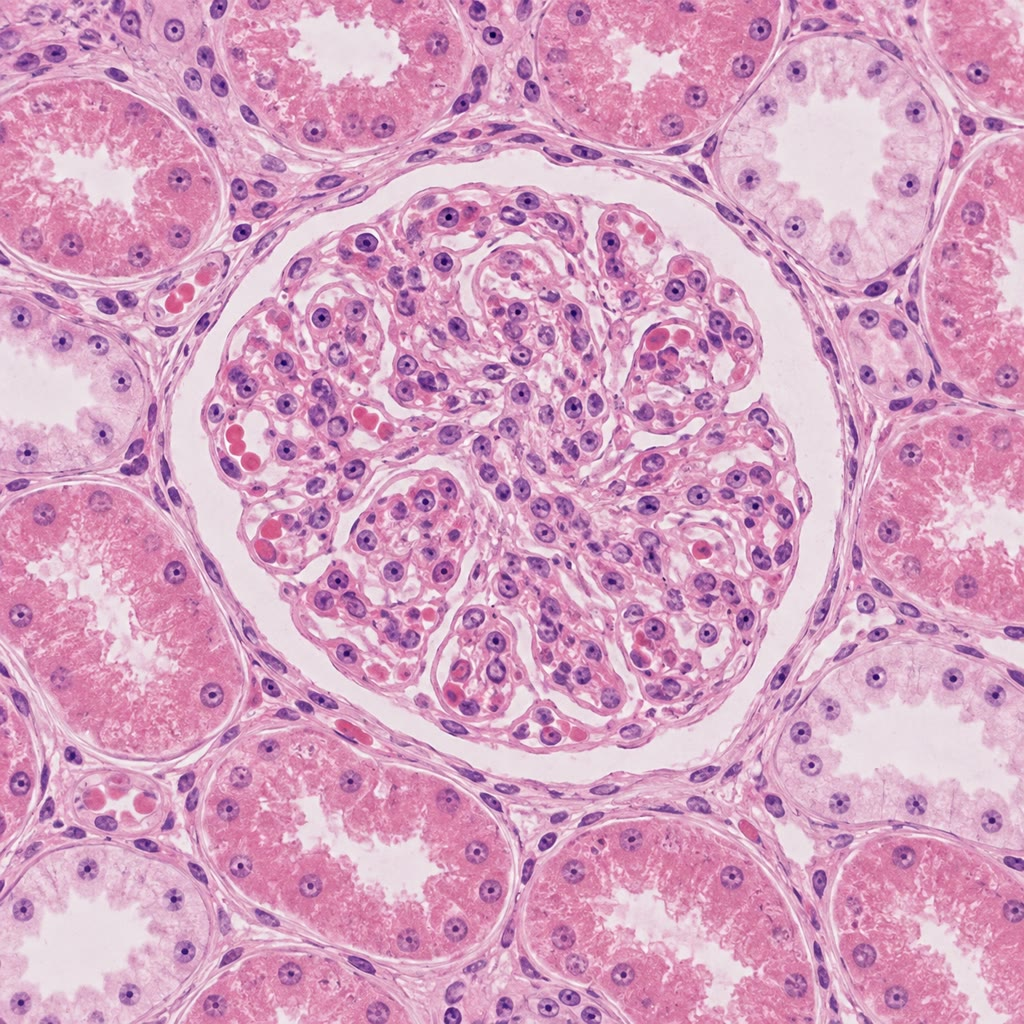
\includegraphics[width=0.46\linewidth]{images/book5/ai/b5-20-kidney-section.jpg}\hspace{0.04\linewidth}
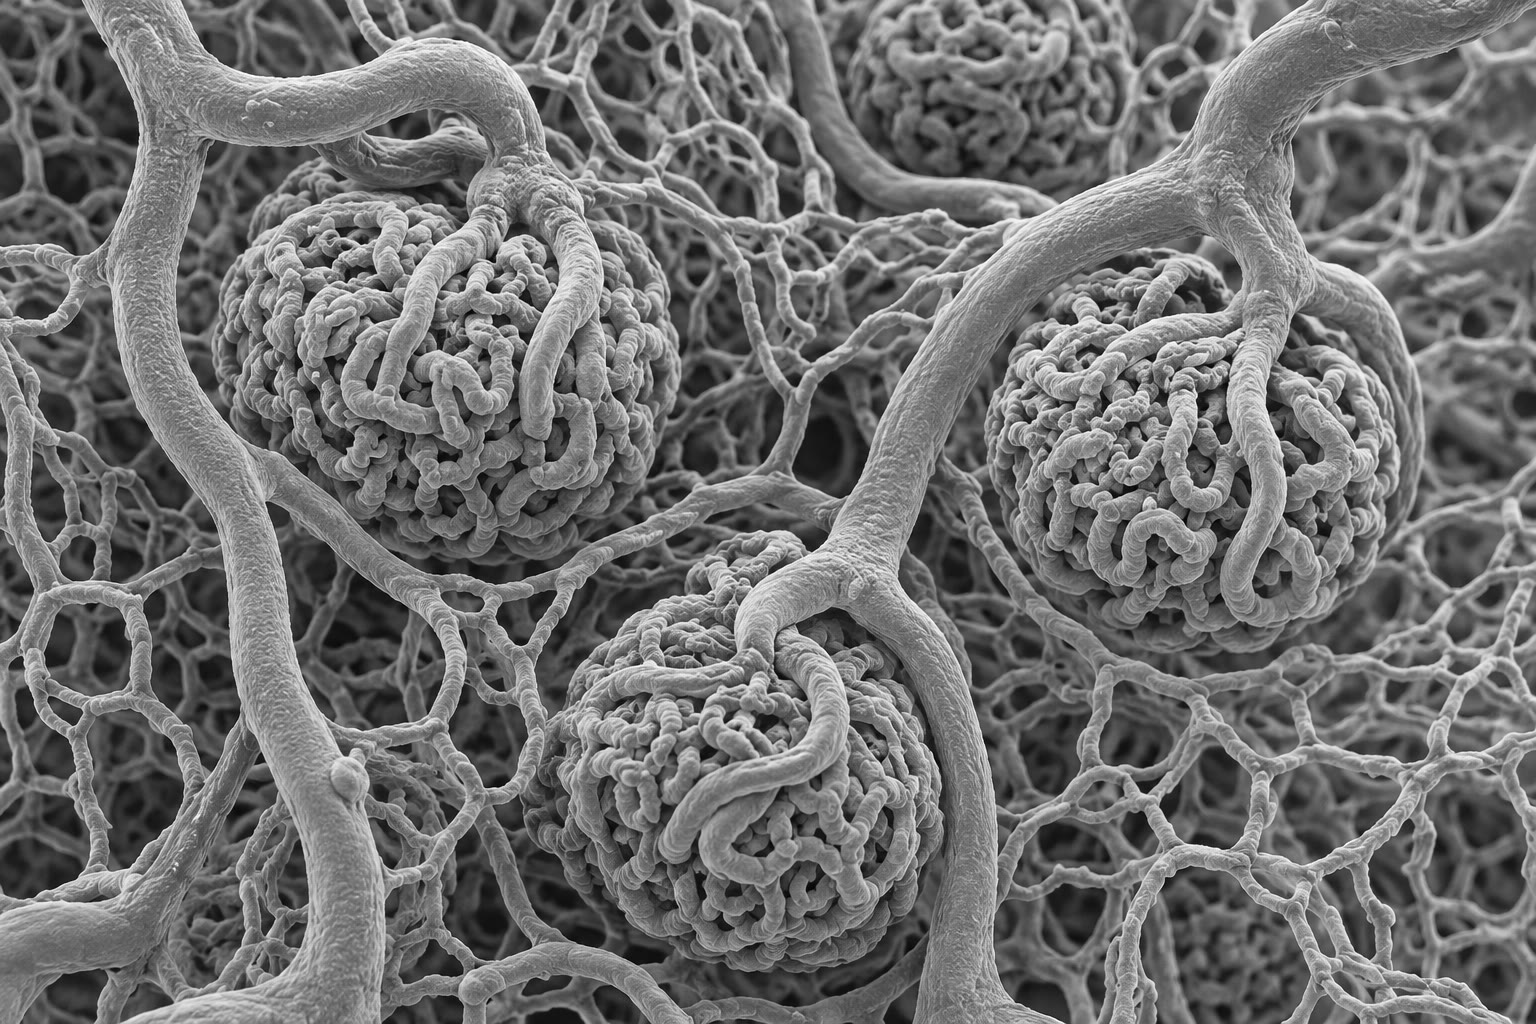
\includegraphics[width=0.46\linewidth]{images/book5/ai/b5-20-nephron-cast.jpg}

{\small Izquierda: corteza renal en corte ---un \omterm{def:b3:renal-osmoregulation:nephron}{glomérulo} en su cápsula
entre los perfiles de los \omterm{def:b3:renal-osmoregulation:nephron}{túbulos proximales} y distales. Derecha: un
molde vascular de la corteza, en el que cada ovillo es un \omterm{def:b3:renal-osmoregulation:nephron}{glomérulo} con
sus vasos aferente y eferente entre los capilares peritubulares.}
\end{omfigure}

\section{Otros animales, otras soluciones}

\begin{definition}[La osmorregulación a lo largo del reino animal]\label{def:b3:renal-osmoregulation:comparative}
\index{túbulo de Malpighi}\index{glándula de la sal}\index{célula de cloruro}\index{agua metabólica}\index{grosor medular relativo}
Los peces de agua dulce viven en un medio de una décima parte de la
\omterm{def:b3:renal-osmoregulation:problem}{osmolaridad} de su sangre: el agua entra a raudales por las branquias,
la sal se escapa, y excretan una orina copiosa y diluida y captan sal
activamente por las \emph{células de cloruro} de las branquias, sin
beber nunca. Los teleósteos marinos, cuya sangre es un tercio de la
\omterm{def:b3:renal-osmoregulation:problem}{osmolaridad} del mar, pierden agua por las branquias, beben agua de mar
y expulsan la sal por esas mismas células de cloruro funcionando al
revés, y mantienen escasa la orina; los tiburones, en cambio, mantienen
su sangre isoosmótica con el mar reteniendo urea (y óxido de
trimetilamina para estabilizar sus proteínas frente a ella), y excretan
el exceso de sal por una glándula rectal. Las aves marinas y los
reptiles marinos llevan \emph{glándulas de la sal} sobre los ojos que
segregan una salmuera dos veces más salada que el mar, lo que permite a
un albatros beber del océano. Los insectos filtran por \emph{túbulos de
Malpighi} impulsados por la secreción activa de potasio y no por la
presión sanguínea, y reabsorben agua en el recto de forma tan completa
que los excrementos de un escarabajo del desierto son secos. Entre los
mamíferos, la capacidad de concentración escala con la longitud de las
asas en relación con el tamaño del riñón (el \emph{grosor medular
relativo}): un castor llega a \qty{500}{mOsm/L}; un ser humano, a
\num{1200}; un camello, a \num{3000}; la rata canguro, a \num{5500}
---lo que le permite vivir del \emph{agua metabólica} liberada cuando
se oxida su alimento, unos \qty{0.6}{g} de agua por gramo de almidón,
con una nariz que recupera el agua de cada espiración por enfriamiento
a contracorriente.
\end{definition}

\begin{omfigure}
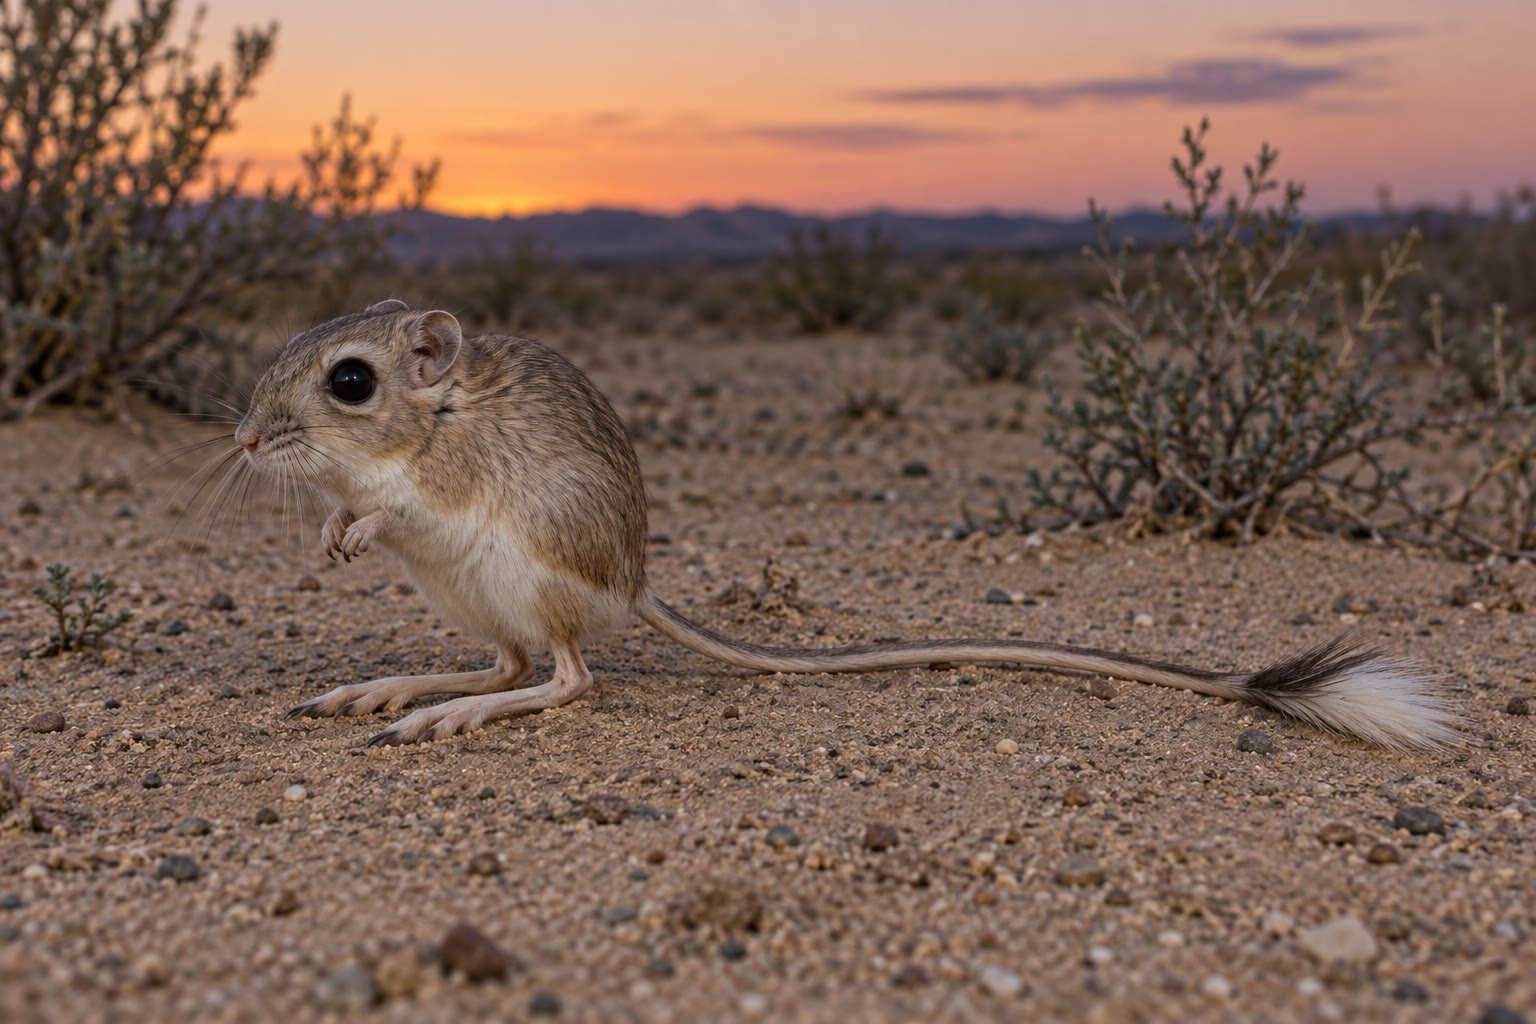
\includegraphics[width=0.56\linewidth]{images/book5/ai/b5-20-kangaroo-rat.jpg}

{\small Una rata canguro, que no bebe nunca: \omterm{def:b3:renal-osmoregulation:nephron}{asas de Henle} largas, una
orina cinco veces más concentrada que el agua de mar, una nariz fría
que condensa el agua de cada respiración y una dieta cuya oxidación
fabrica toda el agua que necesita.}
\end{omfigure}

\begin{remark}[El riñón como problema de diseño]\label{rem:b3:renal-osmoregulation:design}
El riñón de los mamíferos filtra cuarenta veces el volumen plasmático
al día solo para recuperar casi todo: un diseño extravagante, cuyo
sentido es que filtrarlo todo y reabsorber de forma selectiva es más
simple que secretar de forma selectiva cada desecho que pueda aparecer.
Su coste es el \qty{7}{\%} del metabolismo de reposo gastado en
devolver el sodio a bombazos, y su punto débil es el delicado filtro,
que falla despacio bajo una presión alta y una glucosa alta. Su ingenio
es el asa a contracorriente, un recurso que se halla también en las
vejigas natatorias de los peces abisales, en las patas de las aves
zancudas y en las narices de los roedores del desierto, y por el cual
una diferencia local pequeña y asequible se apila hasta formar una
grande ---la misma idea, en cada caso, de que un gradiente puede
construirse a partir del flujo.
\end{remark}

\section{Ejercicios}

\begin{exercise}[$\star$]\label{exo:b3:renal-osmoregulation:1}
Nómbrense en orden los segmentos de la \omterm{def:b3:renal-osmoregulation:nephron}{nefrona} y dígase una cosa que
haga cada uno.
\end{exercise}

\begin{exercise}[$\star$]\label{exo:b3:renal-osmoregulation:2}
Defínase el aclaramiento. Una sustancia tiene una concentración
plasmática de \qty{2}{mg/mL}, una concentración urinaria de
\qty{100}{mg/mL} y el flujo de orina es de \qty{1.5}{mL/min}. Calcúlese
su aclaramiento y dígase si se reabsorbe, se secreta o ni lo uno ni lo
otro, si la TFG es de \qty{120}{mL/min}.
\end{exercise}

\begin{exercise}[$\star$]\label{exo:b3:renal-osmoregulation:3}
¿Por qué un pez de agua dulce no bebe nunca y un pez marino bebe sin
cesar? ¿Qué hacen las branquias en cada caso?
\end{exercise}

\begin{exercise}[$\star$]\label{exo:b3:renal-osmoregulation:4}
¿Cuál es el \omterm{prop:b3:renal-osmoregulation:countercurrent}{efecto simple} del \omterm{def:b3:renal-osmoregulation:nephron}{asa de Henle}, qué rama lo produce y por
qué han de diferir las dos ramas en su permeabilidad al agua?
\end{exercise}

\begin{exercise}[$\star\star$]\label{exo:b3:renal-osmoregulation:5}
Presión capilar glomerular \qty{60}{mmHg}, espacio de Bowman
\qty{18}{mmHg}, presión oncótica plasmática \qty{28}{mmHg} en el
extremo aferente, que sube a \qty{35}{mmHg} en el eferente. Calcúlese
la presión neta de filtración en cada extremo y explíquese por qué la
filtración puede detenerse antes del final del capilar. ¿Qué implica
eso para el efecto del flujo plasmático sobre la TFG?
\end{exercise}

\begin{exercise}[$\star\star$]\label{exo:b3:renal-osmoregulation:6}
El aclaramiento de creatinina de un paciente es de \qty{40}{mL/min}. El
sodio plasmático es \qty{140}{mmol/L}, el sodio urinario
\qty{70}{mmol/L} y el flujo de orina \qty{1}{mL/min}. Calcúlense la
carga filtrada de sodio, la excreción, la fracción reabsorbida y el
aclaramiento de sodio.
\end{exercise}

\begin{exercise}[$\star\star$]\label{exo:b3:renal-osmoregulation:7}
Una persona sigue una dieta que produce \qty{900}{mOsm} de soluto al
día y puede concentrar hasta \qty{1200}{mOsm/L}. ¿Volumen mínimo de
orina? Si una enfermedad renal baja el máximo a \qty{400}{mOsm/L},
¿cuánto debe beber para mantenerse en equilibrio, contando
\qty{0.9}{L} de pérdida insensible?
\end{exercise}

\begin{exercise}[$\star\star$]\label{exo:b3:renal-osmoregulation:8}
Predíganse el volumen y la \omterm{def:b3:renal-osmoregulation:problem}{osmolaridad} de la orina, el sodio plasmático
y el estado de la sed en (a) la diabetes insípida, (b) la secreción
inadecuada de vasopresina por un \omterm{def:b3:cancer-biology:hallmarks}{tumor}, (c) el exceso de \omterm{def:b3:renal-osmoregulation:controls}{aldosterona},
(d) una dieta sin sal durante una semana.
\end{exercise}

\begin{exercise}[$\star\star$]\label{exo:b3:renal-osmoregulation:9}
Calcúlese el \omterm{prop:b3:renal-osmoregulation:water}{aclaramiento de agua libre} para una orina de
\qty{100}{mOsm/L} a \qty{6}{mL/min} y para una orina de
\qty{1000}{mOsm/L} a \qty{0.6}{mL/min}, con el plasma a
\qty{300}{mOsm/L}. Interprétese cada caso.
\end{exercise}

\begin{exercise}[$\star\star\star$]\label{exo:b3:renal-osmoregulation:10}
Modélese el asa como $n$ etapas en las que el líquido ascendente está
en cada etapa \qty{200}{mOsm/L} por debajo del intersticio y el líquido
descendente lo iguala, con el líquido entrando a \qty{300}{mOsm/L}.
Arguméntese que la \omterm{def:b3:renal-osmoregulation:problem}{osmolaridad} en estado estacionario en el recodo
puede acercarse a $300 +
200n$, de modo que el gradiente lo limitan la longitud del asa y el
\omterm{prop:b3:renal-osmoregulation:countercurrent}{efecto simple} de la bomba, y dígase qué fija $n$ físicamente.
\end{exercise}

\begin{exercise}[$\star\star\star$]\label{exo:b3:renal-osmoregulation:11}
Una rata canguro come \qty{5}{g} de semilla seca al día, con un
\qty{80}{\%} de almidón, oxidado a CO$_{2}$ y agua (\qty{0.6}{g} de
agua por gramo de almidón). Debe excretar \qty{3}{mOsm} de soluto al
día a \qty{5500}{mOsm/L}, y pierde \qty{1.5}{g} de agua al día por
evaporación desde una nariz que recupera el \qty{70}{\%} del agua de su
respiración. Hágase el balance de su presupuesto hídrico y dígase si
sobrevive sin beber.
\end{exercise}

\begin{exercise}[$\star\star\star$]\label{exo:b3:renal-osmoregulation:12}
La diálisis hace pasar la sangre por un lado de una membrana y el
líquido de diálisis por el otro, a contracorriente. Explíquese por qué
el flujo a contracorriente depura más que el flujo paralelo, estímese
el aclaramiento de una máquina que retira urea de \qty{300}{mL/min} de
sangre con un rendimiento del \qty{70}{\%}, y compárese con dos riñones
a lo largo de una semana si la máquina funciona cuatro horas tres veces
por semana.
\end{exercise}

\section{Problema: dieciocho cubos al día}

\begin{problem}[{Problema de fin de semana --- el filtrado de un día
seguido del glomérulo a la vejiga: las presiones de Starling, los
aclaramientos de cuatro sustancias, el umbral de la glucosa, el
presupuesto hídrico desde la dilución máxima hasta el agua de mar y el
balance de un roedor del desierto, para terminar en la TFG, el volumen
obligatorio de orina y el agua neta que rinde un litro de agua de
mar}]
\label{pb:b3:renal-osmoregulation:1}
Datos: $K_{f} = \qty{12.5}{mL/min/mmHg}$; $P_{\text{CG}} = \qty{55}{mmHg}$,
$P_{\text{EB}} = \qty{15}{mmHg}$, $\pi_{\text{CG}} = \qty{30}{mmHg}$.
Plasma: inulina \qty{0.5}{mg/mL}, creatinina \qty{0.01}{mg/mL}, urea
\qty{5}{mmol/L}, glucosa \qty{5}{mmol/L}, paraaminohipurato
\qty{0.02}{mg/mL}, Na$^{+}$ \qty{140}{mmol/L}, \omterm{def:b3:renal-osmoregulation:problem}{osmolaridad}
\qty{290}{mOsm/L}. Flujo de orina \qty{1}{mL/min}: inulina
\qty{62.5}{mg/mL}, creatinina \qty{1.3}{mg/mL}, urea \qty{250}{mmol/L},
glucosa $0$, paraaminohipurato \qty{13}{mg/mL}, Na$^{+}$
\qty{100}{mmol/L}, \omterm{def:b3:renal-osmoregulation:problem}{osmolaridad} \qty{600}{mOsm/L}. Hematocrito $0.45$.
Glucosa: $T_{m} =
\qty{375}{mg/min}$ (\qty{2.1}{mmol/min}). Soluto diario \qty{600}{mOsm};
$U_{\max} = \qty{1200}{mOsm/L}$, $U_{\min} = \qty{50}{mOsm/L}$;
pérdida insensible \qty{0.9}{L/d}; agua de mar \qty{1000}{mOsm/L}.

\medskip
\noindent\textbf{Parte I --- El filtro.}
\begin{enumerate}
  \item Calcúlense la presión neta de filtración y la TFG.
  \item Conviértase la TFG a litros por día. ¿Cuántas veces se filtra
        el volumen plasmático (\qty{3}{L})?
  \item Calcúlese el aclaramiento de inulina y compárese con la TFG.
        Calcúlese el aclaramiento de creatinina; ¿por qué es algo
        mayor?
  \item Calcúlense el aclaramiento de paraaminohipurato (el flujo
        plasmático renal), el flujo sanguíneo renal y la fracción de
        filtración.
  \item La arteriola eferente se contrae y eleva $P_{\text{CG}}$ hasta
        \qty{60}{mmHg}. ¿Nueva TFG? ¿Por qué los fármacos que bloquean
        la angiotensina II bajan un poco la TFG en un riñón sano y
        protegen uno diabético?
  \item Aparece proteína en la orina a \qty{3}{g/d}. ¿Qué capa del
        filtro ha fallado, y qué les ocurre a la presión oncótica
        plasmática y a los tejidos si continúa?
\end{enumerate}

\medskip
\noindent\textbf{Parte II --- El manejo.}
\begin{enumerate}[resume]
  \item Urea: carga filtrada, excreción, fracción reabsorbida y
        aclaramiento.
  \item Sodio: carga filtrada por día en moles y en gramos, excreción y
        fracción reabsorbida. ¿Cuántos kilogramos de sal se perderían
        en un día si no se reabsorbiera nada?
  \item Glucosa: carga filtrada en mmol/min y en gramos por día; ¿se
        excreta algo? ¿A qué glucosa plasmática alcanza la carga
        filtrada el $T_{m}$ (el umbral)?
  \item Un diabético tiene una glucosa plasmática de \qty{20}{mmol/L}.
        Glucosa excretada por minuto y por día en gramos, y el volumen
        extra de orina si cada \qty{300}{mOsm} de glucosa arrastra
        \qty{1}{L} a la concentración imperante. Explíquense la sed y
        la pérdida de peso de la diabetes no tratada.
  \item Reabsorber sodio cuesta un ATP por cada tres Na$^{+}$. ¿Cuántos
        moles de ATP al día gasta el riñón en el sodio, y cuántos
        kilojulios (\qty{50}{kJ/mol})? Compárese con los \qty{7}{MJ/d}
        de reposo.
  \item Explíquese por qué el riñón filtra y reabsorbe en lugar de
        secretar cada desecho, en términos de lo que el túbulo tendría
        que reconocer.
\end{enumerate}

\medskip
\noindent\textbf{Parte III --- El agua.}
\begin{enumerate}[resume]
  \item Aclaramiento osmolar $U_{\text{osm}}V/P_{\text{osm}}$ a partir
        de los datos, y \omterm{prop:b3:renal-osmoregulation:water}{aclaramiento de agua libre}. ¿La persona
        conserva agua o la desecha?
  \item Volumen mínimo de orina para el soluto diario; máximo (a
        $U_{\min}$); la necesidad diaria total de agua en el mínimo,
        con la pérdida insensible.
  \item Se bebe un litro de agua de mar. ¿Cuánta orina hace falta para
        excretar su sal a $U_{\max}$, y cuál es la ganancia neta de
        agua antes de contar el soluto propio del día? ¿Y después?
  \item Falta la vasopresina (diabetes insípida) y la orina se queda en
        $U_{\min}$. Volumen diario de orina para el mismo soluto, y
        agua que hay que beber cada día para mantener el equilibrio.
  \item Cerveza a \qty{20}{mOsm/L}: ¿cuánta puede beberse al día antes
        de que el riñón, en $U_{\min}$, ya no pueda excretar el agua?
        (El agua que excede de lo que el soluto puede arrastrar en
        $U_{\min}$ se acumula.)
  \item Tras una noche sin agua la \omterm{def:b3:renal-osmoregulation:problem}{osmolaridad} plasmática es de
        \qty{298}{mOsm/L}. ¿En qué porcentaje ha subido y qué hace el
        hipotálamo? Estímese el déficit de agua si el agua corporal
        total es de \qty{42}{L} y el soluto no ha cambiado.
  \item Explíquese por qué un corredor de maratón que bebe \qty{6}{L}
        de agua mientras suda sal puede desarrollar un sodio plasmático
        peligrosamente bajo, y qué tendría que hacer el riñón para
        impedirlo.
\end{enumerate}

\medskip
\noindent\textbf{Parte IV --- El desierto.}
\begin{enumerate}[resume]
  \item Una rata canguro excreta \qty{3}{mOsm} al día a
        \qty{5500}{mOsm/L}. ¿Volumen de orina? Compárese con el volumen
        que un riñón humano necesitaría para el mismo soluto en su
        propio máximo.
  \item Su alimento rinde \qty{2.4}{g} de \omterm{def:b3:renal-osmoregulation:comparative}{agua metabólica} al día y
        pierde \qty{1.6}{g} al respirar y \qty{0.3}{g} en las heces.
        Hágase el balance con la orina de la pregunta 20.
  \item Un camello concentra hasta \qty{3000}{mOsm/L} y tolera perder
        el \qty{25}{\%} del agua de su cuerpo. Para un camello de
        \qty{500}{kg} con un \qty{65}{\%} de agua, ¿cuánto puede perder
        y cuántos días cubre eso a una pérdida de \qty{5}{L/d}?
  \item Un ave marina come \qty{200}{g} de pescado y bebe \qty{100}{mL}
        de agua de mar al día, con lo que ingiere \qty{150}{mmol} de
        NaCl. Su \omterm{def:b3:renal-osmoregulation:comparative}{glándula de la sal} segrega a \qty{800}{mmol/L}.
        ¿Cuánta salmuera produce, y por qué es la glándula mejor que el
        riñón (que en las aves concentra solo hasta \qty{600}{mOsm/L})
        para esto?
  \item Un pez de agua dulce de \qty{100}{g} gana cada día en agua el
        \qty{30}{\%} de su masa corporal a través de las branquias.
        ¿Cuánta orina debe fabricar, a qué \omterm{def:b3:renal-osmoregulation:problem}{osmolaridad} respecto de su
        sangre, y qué le ocurriría a su sal sin captación activa?
  \item Resúmase: la TFG (pregunta~1), el volumen obligatorio de orina
        (pregunta~14) y el agua neta de un litro de agua de mar después
        de contar el soluto del día (pregunta~15).
\end{enumerate}
\end{problem}
